\textbf{Objetivo}

El objetivo de esta práctica es que el alumno comprenda los aspectos principales acerca de la estructura del sistema Operativo GNU/Linux en lo que respecta a procesos, usuarios, filesystems, permisos, etc.

\begin{questions}

\question Editor de textos:
\begin{parts}
	\part Nombre al menos 3 editores de texto que puede utilizar desde linea de comandos.
	\part ¿En que se diferencia un editor de texto a los comandos cat, more o less? Enumere los modos de operación que posee el editor de textos vi.
 	\part Nombre los comandos mas comunes que se le pueden enviar al editor de textos vi.
\end{parts}

\question Proceso de Arranque \textit{SystemV}:
\begin{parts}
	\part Enumere los pasos del proceso de inicio de un sistema GNU/Linux, desde que se prende la PC hasta que se logra obtener el login en el sistema.
 	\part Proceso \textbf{INIT}. ¿Quién lo ejecuta? ¿Cuál es su objetivo?
 	\part Ejecute el comando pstree. ¿Que es lo que se puede observar a partir de la ejecución de este comando?.
 	\part RunLevels. ¿Qué son? ¿Cuál es su objetivo?
 	\part ¿A qué hace referencia cada nivel de ejecución según el estándar? ¿Dónde se define que Runlevel ejecutar al iniciar el sistema operativo? ¿todas las distribuciones respetan estos estándares?
	\part Archivo /etc/inittab. ¿Cuál es su finalidad? ¿Qué tipo de información se almacena en el? ¿Cuál es la estructura de la información que en el se almacena?
 	\part	Suponga que se encuentra en el runlevel <X>. Indique qué comando(s) ejecutaría para cambiar al runlevel <Y>. ¿Este cambio es permanente? ¿Por qué?
 	\part Scripts RC. ¿Cuál es su finalidad? ¿Dónde se almacenan? Cuando un sistema GNU/Linux arranca o se detiene se ejecutan scripts, indique como determina que script ejecutar ante cada acción. ¿Existe un orden para llamarlos? Justifique.
 	\part ¿Qué es insserv? ¿Para qué se utiliza? ¿Qué ventajas provee respecto de un arranque tradicional?
 	\part ¿Cómo maneja Upstart el proceso de arranque del sistema?
 	\part Cite las principales diferencias entre SystemV y Upstart.
	\part Que reemplaza a los script \textit{rc} de \textit{SystemV} en \textit{Upstart}? En que ubicación se encuentran?
	\part Dado el siguiente \textit{job} de upstart perteneciente al servicio de base de datos del mysql indique a que hace referencia cada linea del mismo:
	\begin{lstlisting}
# MySQL Service
description "MySQL Server"
author "info autor"
start on (net-device-up
	and local-filesystems
	and runlevel [2345])
stop on runlevel [016]

[...]
exec /usr/sbin/mysqld
[...]
	\end{lstlisting}

	\part ¿Que es \textit{sytemd}?
	\part ¿A que hace referencia el concepto de activación de socket en \text{systemd}?
	\part ¿A que hace referencia el concepto de \textit{cgroup}?
\end{parts}

\question Usuarios:
\begin{parts}
	\part ¿Qué archivos son utilizados en un sistema GNU/Linux para guardar la información de los usuarios?
	\part ¿A que hacen referencia las siglas \textit{UID} y \textit{GID}? ¿Pueden coexistir UIDs iguales en un sistema GNU/Linux? Justifique.
	\part ¿Qué es el usuario root? ¿Puede existir más de un usuario con este perfil en GNU/Linux? ¿Cuál es la \textit{UID} del \textit{root}?.
	\part Agregue un nuevo usuario llamado iso2015 a su instalación de GNU/Linux, especifique que su home sea creada en /home/iso\_2015, y hágalo miembro del grupo cátedra (si no existe, deberá crearlo). Luego, sin iniciar sesión como este usuario cree un archivo en su home personal que le pertenezca. Luego de todo esto, borre el usuario y verifique que no queden registros de él en los archivos de información de los usuarios y grupos.
	\part Investigue la funcionalidad y parámetros de los siguientes comandos:
	\begin{itemize}
		\item useradd ó adduser
		\item usermod
		\item userdel
		\item su
		\item groupadd
		\item who
		\item groupdel
		\item passwd
	\end{itemize}
\end{parts}

\question FileSystem:
\begin{parts}
	\part ¿Cómo son definidos los permisos sobre archivos en un sistema GNU/Linux?
	\part Investigue la funcionalidad y parámetros de los siguientes comandos relacionados con los permisos en GNU/Linux:
	\begin{itemize}
		\item chmod
		\item chown
		\item chgrp
	\end{itemize}
	\part Al utilizar el comando chmod generalmente se utiliza una notación octal asociada para definir permisos. ¿Qué significa esto? ¿A qué hace referencia cada valor?
	\part ¿Existe la posibilidad de que algún usuario del sistema pueda acceder a determinado archivo para el cual no posee permisos? Nombrelo, y realice las pruebas correspondientes.
	\part Explique los conceptos de “full path name” y “relative path name”. De ejemplos claros de cada uno de ellos.
	\part ¿Con qué comando puede determinar en qué directorio se encuentra actualmente? ¿Existe alguna forma de ingresar a su directorio personal sin necesidad de escribir todo el path completo? ¿Podría utilizar la misma idea para acceder a otros directorios? ¿Cómo? Explique con un ejemplo.
	\part Investigue la funcionalidad y parámetros de los siguientes comandos relacionados con el uso del FileSystem:
	\begin{itemize}
		\item cd
		\item umount
		\item mkdir
		\item du
		\item rmdir
		\item df
		\item mount
		\item ln
		\item ls
		\item pwd
		\item cp
		\item mv
	\end{itemize}
\end{parts}

\question Procesos:
\begin{parts}
	\part ¿Qué es un proceso? ¿A que hacen referencia las siglas \textit{PID} y \textit{PPID}? ¿Todos los procesos tienen estos atributos en GNU/Linux? Justifique. Indique que otros atributos tiene un proceso.
	\part Indique que comandos se podrían utilizar para ver que procesos están en ejecución en un sistema GNU/Linux.
	\part ¿Qué significa que un proceso se esta ejecutando en Background? ¿Y en Foreground?
	\part ¿Cómo puedo hacer para ejecutar un proceso en Background? ¿Como puedo hacer para pasar un proceso de background a foreground y viceversa?
	\part Pipe ( \textbf{|} ). ¿Cual es su finalidad? Cite ejemplos de su utilización.
	\part Redirección. ¿Qué tipo de redirecciones existen? ¿Cuál es su finalidad? Cite ejemplos de utilización.
	\part Comando \textit{kill}. ¿Cuál es su funcionalidad? Cite ejemplos.
	\part Investigue la funcionalidad y parámetros de los siguientes comandos relacionados con el manejo de procesos en GNU/Linux. Además
	compárelos entre ellos:
	\begin{itemize}
		\item ps
		\item kill
		\item pstree
		\item killall
		\item top
		\item nice
	\end{itemize}
\end{parts}

\question Otros comandos de Linux (Indique funcionalidad y parámetros):
\begin{parts}
	\part ¿A qué hace referencia el concepto de empaquetar archivos en GNU/linux?
	\part Seleccione 4 archivos dentro de algún directorio al que tenga persmiso y sume el tamaño de cada uno de estor archivos. Cree un archivo empaquetado conteniendo estos 4 archivos y compare los tamaños de los mismos. ¿Qué característica nota?
	\part ¿Qué acciones debe llevar a cabo para comprimir 4 archivos en uno solo? Indique la secuencia de comandos ejecutados.
	\part ¿Pueden comprimirse un conjunto de archivos utilizando un único comando?
	\part Investigue la funcionalidad de los siguientes comandos:
	\begin{itemize}
		\item tar
		\item grep
		\item gzip
		\item zgrep
		\item wc
	\end{itemize}
\end{parts}

\question Indique que acción realiza cada uno de los comandos indicados a continuación considerando su orden. Suponga que se ejecutan desde un usuario que no es root ni pertenece al grupo de root. (Asuma que se encuentra posicionado en el directorio de trabajo del usuario con el que se logueo). En caso de no poder ejecutarse el comando indique la razón:
\begin{lstlisting}
		ls -l > prueba
		ps > PRUEBA
		chmod 710 prueba
		chown root:root PRUEBA
		chmod 777 PRUEBA
		chmod 700 /etc/passwd
		passwd root
		rm PRUEBA
		man /etc/shadow
		find / -name *.conf
		usermod root -d /home/newroot -L
		cd /root
		rm *
		cd /etc
		cp * /home -R
		shutdown
\end{lstlisting}

\question Indique que comando seria necesario ejecutar para realizar cada una de las siguientes acciones:
\begin{parts}
	\part Terminar el proceso con \textit{PID} 23.
	\part Terminar el proceso llamado \textit{init}. ¿Qué resultados obtuvo?
	\part Buscar todos los archivos de usuarios en los que su nombre contiene la cadena “.conf”
	\part Guardar una lista de procesos en ejecución el archivo \textbf{/home/<su nombre de usuario>/procesos}
	\part Cambiar los permisos del archivo \textbf{/home/<su nombre de usuario>/xxxx} a:
	\begin{itemize}
		\item Usuario: Lectura, escritura, ejecución
		\item Grupo: Lectura, ejecución
		\item Otros: ejecución
	\end{itemize}
	\part Cambiar los permisos del archivo \textbf{/home/<su nombre de usuario>/yyyy} a:
	\begin{itemize}
		\item Usuario: Lectura, escritura.
		\item Grupo: Lectura, ejecución
		\item Otros: Ninguno
	\end{itemize}
	\part Borrar todos los archivos del directorio \textbf{/tmp}
	\part Cambiar el propietario del archivo \textbf{/opt/isodata} al usuario \textbf{iso2010}
	\part Guardar en el archivo \textbf{/home/<su nombre de usuario>/donde} el directorio donde me encuentro en este momento, en caso de que el archivo exista no se debe eliminar su contenido anterior.
\end{parts}

\question Indique que comando seria necesario ejecutar para realizar cada una de las siguientes acciones:
\begin{parts}
	\part Ingrese al sistema como usuario “root”
	\part Cree un usuario. Elija para como nombre, por convención, la primer letra de su nombre seguida de su apellido. Asígnele una contraseña de acceso.
 	\part ¿Qué archivos fueron modificados luego de crear el usuario y qué directorios se crearon?
	\part Crear un directorio en /tmp llamado cursada2010
	\part Copiar todos los archivos de /var/log al directorio antes creado.
	\part Para el directorio antes creado (y los archivos y subdirectorios contenidos en él) cambiar el propietario y grupo al usuario creado y grupo users.
	\part Agregue permiso total al dueño, de escritura al grupo y escritura y ejecución a todos los demás usuarios para todos los archivos dentro de un directorio en forma recursiva.
	\part Acceda a otra terminal virtual para loguearse con el usuario antes creado.
	\part Una vez logueado con el usuario antes creado, averigüe cual es el nombre de su terminal.
	\part Verifique la cantidad de procesos activos que hay en el sistema.
	\part Verifiqué la cantidad de usuarios conectados al sistema.
	\part Vuelva a la terminal del usuario root, y envíele un mensaje al usuario anteriormente creado, avisándole que el sistema va a ser apagado.
	\part Apague el sistema.
\end{parts}

\question Indique que comando seria necesario ejecutar para realizar cada una de las siguientes acciones:
\begin{parts}
	\part Cree un directorio cuyo nombre sea su número de legajo e ingrese a él.
	\part Cree un archivo utilizando el editor de textos vi, e introduzca su información personal: Nombre, Apellido, Número de alumno y dirección de correo electrónico. El archivo debe llamarse "LEAME".
	\part Cambie los permisos del archivo LEAME, de manera que se puedan ver reflejados los siguientes permisos:
	\begin{itemize}
		\item Dueño: ningún permiso
		\item Grupo: permiso de ejecución
		\item Otros: todos los permisos
	\end{itemize}
	\part Vaya al directorio /etc y verifique su contenido. Cree un archivo dentro de su directorio personal cuyo nombre sea leame donde el contenido del mismo sea el listado de todos los archivos y directorios contenidos en /etc. ¿Cuál es la razón por la cuál puede crear este archivo si ya existe un archivo llamado "LEAME" en este directorio?.
	\part ¿Qué comando utilizaría y de qué manera si tuviera que localizar un archivo dentro del file system? ¿Y si tuviera que localizar varios archivos con características similares? Explique el concepto teórico y ejemplifique.
	\part Utilizando los conceptos aprendidos en el punto e), busque todos los archivos cuya extensión sea .so y almacene el resultado de esta búsqueda en un archivo dentro del directorio creado en a). El archivo deberá llamarse "ejercicio\_f".
\end{parts}

\question Indique que acción realiza cada uno de los comandos indicados a continuación considerando su orden. Suponga que se ejecutan desde un usuario que no es root ni pertenece al grupo de root. (Asuma que se encuentra posicionado en el directorio de trabajo del usuario con el que se logueó). En caso de no poder ejecutarse el comando indique la razón:
\begin{lstlisting}
	mkdir iso
	cd ./iso; ps > f0
	ls > f1
	cd /
	echo $HOME
	ls -l $> $HOME/iso/ls
	cd $HOME; mkdir f2
	ls -ld f2
	chmod 341 f2
	touch dir
	cd f2
	cd ~/iso
	pwd >f3
	ps | grep 'ps' | wc -l >> ../f2/f3
	chmod 700 ../f2; cd ..
	find . -name etc/passwd
	find / -name etc/passwd
	mkdir ejercicio5
	..................................................
	..................................................
\end{lstlisting}
\begin{parts}
	\part Inicie 2 sesiones utilizando su nombre de usuario y contraseña. En una sesión vaya siguiendo paso a paso las órdenes que se encuentran escritas en el cuadro superior. En la otra sesión, cree utilizando algún editor de textos un archivo que se llame "ejercicio10\_explicacion" dentro del directorio creado en el ejercicio 9.a) y, para cada una de las órdenes que ejecute en la otra sesión, realice una breve explicación de los resultados obtenidos.
	\part Complete en el cuadro superior los comandos 19 y 20, de manera tal que realicen la siguiente acción:
	\begin{itemize}
		\item 19: Copiar el directorio iso y todo su contenido al directorio creado en el inciso 9.a).
		\item 20: Copiar el resto de los archivos y directorios que se crearon en este ejercicio al directorio creado en el ejercicio 9.a).
	\end{itemize}
	\part Ejecute las órdenes 19 y 20 y comentelas en el archivo creado en el inciso a).
\end{parts}

\question Cree una estructura desde el directorio /home que incluya varios directorios, subdirectorios y archivos, según el esquema siguiente. Asuma que “usuario” indica cuál es su nombre de usuario. Además deberá tener en cuenta que dirX hace referencia a directorios y fX hace referencia a archivos:
\begin{figure}
	\centering
	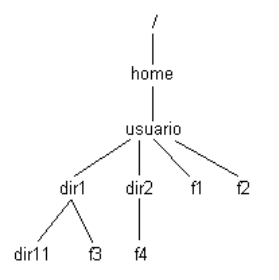
\includegraphics[scale=0.5]{images/ejer12.png}
\end{figure}
\begin{parts}
	\part	Utilizando la estructura de directorios anteriormente creada, indique que comandos son necesarios para realizar las siguientes acciones:
\end{parts}
\begin{itemize}
	\item Mueva el archivo "f3" al directorio de trabajo /home/usuario.
	\item Copie el archivo "f4" en el directorio "dir11".
	\item Haga los mismo que en el inciso anterior pero el archivo de destino, se debe llamar "f7".
	\item Cree el directorio copia dentro del directorio usuario y copie en él, el contenido de "dir1".
	\item Renombre el archivo "f1" por el nombre archivo y vea los permisos del mismo.
	\item Cambie los permisos del archivo llamado archivo de manera de reflejar lo siguiente:
	\begin{itemize}
		\item Usuario: Permisos de lectura y escritura
		\item Grupo: Permisos de ejecución
		\item Otros: Todos los permisos
	\end{itemize}
	\item Renombre los archivos "f3" y "f4" de manera que se llamen "f3.exe" y "f4.exe" respectivamente.
	\item	Utilizando un único comando cambie los permisos de los dos archivos renombrados en el inciso anterior, de manera de reflejar lo siguiente:
	\begin{itemize}
		\item Usuario: Ningún permiso
		\item Grupo: Permisos de escritura
		\item Otros: Permisos de escritura y ejecución
	\end{itemize}
\end{itemize}

\question Indique que comando/s es necesario para realizar cada una de las acciones de la siguiente secuencia de pasos (considerando su orden de aparición):
\begin{parts}
	\part Cree un directorio llamado logs en el directorio /tmp.
	\part Copie todo el contenido del directorio /var/log en el directorio creado en el punto anterior.
	\part Empaquete el directorio creado en 1, el archivo resultante se debe llamar "misLogs.tar".
	\part Empaquete y comprima el directorio creado en 1, el archivo resultante se debe llamar "misLogs.tar.gz".
	\part Copie los archivos creados en 3 y 4 al directorio de trabajo de su usuario.
	\part Elimine el directorio creado en 1, logs.
	\part Desempaquete los archivos creados en 3 y 4 en 2 directorios diferentes.
\end{parts}

\end{questions}
